\chapter{Analysis and Interpretation of Results}

This section addresses mainly the RQ3. The type of hashtags recommendation used is proposing a prediction study that is content based for government tweet content, an approach using LDA Topic modelling.  This chapter outlines the experimental design explaining how the study is carried out for ultimate prediction techniques and comparisons of the prediction models. Therefore, the chapter will cover 3 phases, starting with preparation of source data, followed by text mining prediction techniques encompassing supervised and unsupervised models and last the evaluation of models. 

In the advertising of products various recommendation methods have been proposed to predict the wanted products based on users’ preferences as well as preferences for similar users [12]. 

To make an attempt to predict hashtags recommendation the approach used is text based methods.   The two models to be discussed for hashtag recommendation of tweets is the unsupervised LDA topic based model, as well as supervised prediction techniques encompassing Random Forest Classifier (RFC) and Support Vector Machine Classifier (SVC).  

The model evaluation techniques to compare model performance conducted for both supervised and unsupervised methods is the accuracy score.  

\section{Data Preparation}

Tweet text posted on "sarstax" were extracted for the following period, considering the keywords "sarstax".
"Converting unstructured data into structured data by collecting data from sources like plain text, web pages and data files."

These are tweets emanating from the revenue government for the four year period, 2018 - 2021 forming a data set of 7 877 without retweets.

The data description for the 4 years amounted to 65 919 entries and 34 features, with the same number of data features as the government tweets (??to verify this with some literature) including for those not populated.

\section{Software}

The analysis was conducted in Python environment, version 3.9 and using Jupyter Notebook to write and develop all the python code data analysis scripts.  The Python environment comes with 3rd party libraries offering tool its for all python tasks from data sourcing, preparation, processing, text analysis and visualization.   
\section{Pre-Processing}

In order to cleanse, remove ad detect anomalies the following pre-processing steps have been applied which include:
\begin{itemize}
    \item Normalization to put all text on the same level,
    such as lower case, remove special characters, remove stopwords, all this to improve text matching.
\end{itemize}
\begin{itemize}
    \item removing retweets  characters
\end{itemize}
\begin{itemize}
    \item Removal of english stop words that have low content discriminative value.  Also removal of additional words relating to the tax environment. 
\end{itemize}
\begin{itemize}
    \item Any other noise such removal of hyperlinks, HTML tags,symbols, punctuation marks, etc.
\end{itemize}
\begin{itemize}
    \item Replaced contractions of words to minimize shortness of already short text tweets
\end{itemize}
\begin{itemize}
    \item Lemmatization to reduce words to root words for production of tokens.
\end{itemize}
\begin{itemize}
    \item Tokenization: The tokenized text is contained in a Document-Term Matrix of a dictionary containing unique words with those less than 3 in length deleted.
\end{itemize}
\begin{itemize}
    \item the data pre-processing ends with vectorizing to convert the bag of words to numbers for machine learning modelling.  The method used is created from an intensified dictionary having applied TF-IDF vectorization technique to systematically increase usage of importance words in the document.  "TF-IDF refers to Term Frequency Inverse Document Frequency for a numerical statistic measure used to score the importance of a word in any content collection of documents and it checks how relevant the word is in the corpus. This process not only considers the frequency but also induces discriminative information for each term.
\end{itemize}

Overall, for the prediction technique is applied to tweets with identified hashtags for the labeled 
\begin{itemize}
    \item Total number of words: 104987 words.
\end{itemize}
\begin{itemize}
    \item Mean number of words per tweet: 13.33 words.
\end{itemize}
\begin{itemize}
    \item Total length of the data set is: 761 122 characters.
\end{itemize}
\begin{itemize}
    \item Mean length of a tweet is: 97.0.
\end{itemize}

The next step is to investigate on the feature extraction process as an input document word matrix for the LDA topic model parameter is an encoded vectorized words for each individual tweet using the TFIDF Vectorizer approach that provides better interpretation of resulting topics, hopefully an approach to find relevance between hashtags and tweets.  [14]The TFIDF Vectorizer output is in the form of a sparse matrix, therefore calculating sparsicity as the percentage of non-zero cells for the doc-word-matrix is also important to understand the quality of overall data for short texts.  

To fit the training data and transform the training data with the TFIDF Vectorizer, without re-fitting the vectorizer when transforming the test data set.  By fitting means careful consideration of words to consider document quality by further filtering by removing any words that appear in more than 90 percent of tweets (max_df=0.9) deemed to be too common for meaningful in topics. There has been no discard of low appearing words.

So therefore the LDA algorithm model object holds parameters such as the number of topics  in fitting method which will hold fitted parameters which tell us how important different words are in different topics. To also print tf_feature_names to see what tokens made it through filtering.

\textbf{"Note that the tf matrix is exactly like the hashtag_vector_df dataframe. Each row is a tweet and each column is a word. The numbers in each position tell us how many times this word appears in this tweet."}

Next we actually create the model object. Lets start by arbitrarily choosing 10 topics. We also define the random state so that this model is reproducible: lda_model = 
LatentDirichletAllocation(batch_size=128,          doc_topic_prior=None,
evaluate_every=-1, learning_decay=0.7,
                          learning_method='online', learning_offset=50.0,
                          max_doc_update_iter=100, max_iter=5,
                          mean_change_tol=0.001, n_components=10, n_jobs=None,
                          perp_tol=0.1, random_state=0, topic_word_prior=None,
                          total_samples=1000000.0, verbose=0)

To visualize the LDA model outputs through the pyLDAvis python library that enables dynamic exploration of topics by adjusting interactively parameters for enhanced understanding of topic outputs   The visualization of the model output is presented below:

\subsubsection{Data Visualisation of LDA Topic Modelling}\\
The LDA model is useful for accurate formulation of meaningful latent topics even for a short texts contents.  A further step is to visualise the explored topics as an indication that the model is doing well extrapolating distinct topics.  The visualised output of topics in an interactive representation of topics through the pyLDAvis library function available in Python, which gives a good picture of the LDA trained model for the human eye processing.  In addition to processing the topics outputs consideration of topic weights and word distribution rely on the evaluation metrics such as topic interpretability.   Further, the pyLDAvis function provides more parameters that are useful for exploring topic modeling performance and indication of no overlapping topics.  

This is made possible by the following model attributes.
The important metrics to evaluate results for the trained LDA model is measure of perplexity which is indicated to be 0,1.  Amongst important parameters for the trained model is number of topics (k) inline to the perplexity metrics which shows a k value of 10.  

\textbf{Topic evaluation aids deeper understanding to gain insights by navigating through the topics from textual data and facilitates the interpretation and analysis of discovered topics.  By the LDA model visualization through the pyLDAvis function also visible shows important parameters to understand overlapping topics.}

\section{Data Modelling for hashtag recommendation}\\

Overall the corpora is treated labeled for the analysis task of hashtags prediction as it only considers tweets with existing hashtags to have two important variables, hashtag(label) and tokens for the feature vector.  The input feature vector document has a sparsicity value of 0,567.  In preparation to train the classifier the established labeled dataset is randomly split it into two datasets, 70 percent of the data is training set for a model, the remaining 30 percent is a testing set.  Overall data set of 7 856 tweets with labeled hashtags means 5 499 is training and 2 357 test cases used for a quantitative analysis that predicts hashtags using both supervised and unsupervised techniques which are observed and explained below.

\subsection{The general LDA Topic modelling}\\

As mentioned previously, LDA is a generative statistical model to discover probabilistic topics within a collection of documents of aggregated tweets. The LDA model has been employed to identify latent topic presentation of tweets text data and further for recommendation of hashtags system that follow a content based approach.

Topic Model is more powerful that the word cloud (or tag cloud) as it shows which words co-occur in the same documents, with the Latent Dirichlet Allocation or LDA being the most common topic modeling algorithm.  Since the topic modeling is non-deterministic and can offer slightly different topics each time the code is run, the computer's random seed set to equal to 0 in order to get the same results. 

As shown by RQ2 there are meaningful results from the unsupervised training process for LDA Topic modelling since it is well known for its good performance and no association with over-fitting.

In building a base model for the unsupervised model one must have in mind evaluation techniques in choosing the best parameters for the final LDA model.  The process begins with building a default LDA modeL using the Gensim approach, a library in python efficient for required outputs for an iterative tuning of hyper parameters for the final model. 

In order to train the unsupervised base LDA model one must be aware of required inputs which starts with an input text converted into a sparse matrix dictionary that are outcomes of data processing, for the study this is measured sparsicity of 0,567.  The second model input is the number of topics with a default value of 10.  The first iteration of the base LDA model outcomes results includes coherence score useful to measure performance of the model, while also assisting in the iterative process to determine model hyperparameters, which are the number of topics(k), 
Dirichlet hyperparameter alpha (Document-Topic Density), and,
Dirichlet hyperparameter beta (Word-Topic Density).  

"This limitation of perplexity measure served as a motivation for more work trying to model the human judgment, and thus Topic Coherence."  The coherence measure used is C_v,  "the C_v measure is based on a sliding window, one-set segmentation of the top words and an indirect confirmation measure that uses normalized point wise mutual information (NPMI) and the cosine similarity."

"With the coherence score seems to keep increasing with the number of topics, it may make better sense to pick the model that gave the highest C_V before flattening out or a major drop. In this case, we picked K=10.  Next, we want to select the optimal alpha and beta parameters. While there are other sophisticated approaches to tackle the selection process, for this tutorial, we choose the values that yielded maximum C_v score for K=10"

"Let’s train the final model using the above selected parameters"

Therefore, training the final LDA base model using the above selected tested and fine tuned parameters results in final model for use in unsupervised and supervised techniques for hashtag recommendations.
num_topics = 8

[Latent Dirichlet Allocation], Overall with the model results means the LDA model is capable to model each topic (as an infinite mixture over an underlying set of topic probabilities.) distinctly, with documents of a corpus are the observed variable while the structure of the topic, distribution of words in a topic and distribution of topics in a documents is a hidden parameter.  

Latent Dirichlet Allocation is the most popular technique for performing topic modeling. LDA is a probabilistic matrix factorization approach.

To perform the Latent Dirichlet Allocation (LDA) for topic modeling using Scikit-learn, Scikit-learn offers LatentDirichletAllocation for performing LDA on any Document Term Matrix(DTM), that is from sklearn.decomposition import LatentDirichletAllocation

The focus of the experiment is on comparing the performance of LDA Topic modeling against supervised techniques (SVM and RF classifiers) for hashtag recommendation.

\subsubsection{Model evaluation for LDA Topic modelling }\\

Since the research design follows a content based method for hashtag recommendation, a general topics method of the LDA model approach in the experiment, this section covers the evaluation process for models used.   The LDA evaluation method can be computationally expensive is important and covers metric results for quantitative measures demonstrating topic interpretability (coherence, perplexity, etc) and model pre-defining tasks for the prediction required in the hashtag recommendation system.  

[Annexure 1: Output of the perplexity and log-likelihood].  This is accomplished when training the topic model that through iterations of various values for maximum number of topics k, the best LDA model parameters is guided by the performance of perplexity and log-likelihood results.  Therefore in choosing the best LDA model parameters for training one  that converges to suggest a number of hashtags per tweet and captured the general topic of the tweet with suggested perplexity score of 0,1 for minimum topics of 10 and a learning decay of 0.7.  
Overall, described below are the quantitative measures to evaluate the LDA model cover both the training and testing phase of the model building process:

\begin{enumerate}
    \item Number of topics: While in building the trained unsupervised LDA topic modeling method requires an upfront knowledge of important parameter the number of topics (k) of k=10  was used.  The output results of the final model parameters also indicate the no-of-components = 10, therefore no of topics =10 for final.
    \item Topic Coherence: 0,3776 to measure overall coherence between topics inferred by the model.   
    \item Perplexity Score: 0.1 measures values of log-likelihood and perplexity performance scores, the lower perplexity value is considered to be a good model.   
\end{enumerate}

Based on the sampled data sets, Overall performance for the training and testing data sets indicate that fair distribution of hashtags in both data sets.Therefore, With a threshold of 0.010, test set output for hashtags has a distribution resembling results of the training model.  Overall the percentage of posts that have recommended hashtags in the test set with a threshold of 0.010 is 50, thus, producing the highest results.

Average number of hashtags in the training set: 59.83
Median number of hashtags in the training set:  58.0
--------------------------------------
Average number of hashtags in the test set, with a threshold of 0.010: 1.88
Median number of hashtags in the test set, with a threshold of 0.010: 1
Percentage of posts that have recommended hashtags in the test set, with a threshold of 0.010: 72
--------------------------------------
Average number of hashtags in the test set, with a threshold of 0.011: 1.57
Median number of hashtags in the test set, with a threshold of 0.011: 1
Percentage of posts that have recommended hashtags in the test set, with a threshold of 0.011: 65
--------------------------------------
Average number of hashtags in the test set, with a threshold of 0.012: 1.28
Median number of hashtags in the test set, with a threshold of 0.012: 1
Percentage of posts that have recommended hashtags in the test set, with a threshold of 0.012: 57
--------------------------------------
Average number of hashtags in the test set, with a threshold of 0.013: 1.02
Median number of hashtags in the test set, with a threshold of 0.013: 0
Percentage of posts that have recommended hashtags in the test set, with a threshold of 0.013: 49
-------------------------------------- 
    
\subsection{The Prediction LDA Modelling}

The results shown above indicate that an optimized LDA model process as an important process to employ finely tuned  model parameters in building the content based hashthag recommendation model, which is a predictive technique for the hashtag recommendation system based. 

Therefore the prediction of hashtags for recommendation is the final stage culminating from the optimised LDA based model that can suggest valid hashtags for a new data set.  The prediction model employed in the study for LDA prediction is made possible by a built in python library within scikit class, described as sklearn.decomposition.LatentDirichletAllocation, for the purpose model of hashtag recommendation using a text based method.  

 Below are the first results of the recommendation system for twitter user text posts based on a lda model, this system returns up to 5 tags per tweet (user).  

\begin{table}
    \centering
    \begin{tabular}{0.010|0.011|0.012|0.013}
         &[] &[] &[] &[]\\
         [return, file, season, filing]& [return, file, season, filing]& [return, file, season]& [return, file, season]&\\
         [trade, criminal, illicit]& [trade]& [trade]&  [trade]&\\
         []&  []&  []&  []& \\
         [say]& []& []& []&\\
         [call, service, join, revenue]&	[call, service, join]&	[call, service]&	[call, service]& 
         [return]& []& []& []&\\
         []& []& []& []&
         \end{tabular}
    \caption{Caption}
    \label{tab:my_label}
\end{table}

For the threshold of 0.010 the finally results of the recommender system using the lda mthod for prediction of up to 5 hashtags

\begin{table}
    \centering
    \begin{tabular}{c}
        [do, well, campaign, government]\\
        [employer]\\
        [know]\\
        [say]\\
        [act, address, cigarette]\\
        []\\
        [watch, budget,bill,finance,return]\\
        [cigarette, trade]\\
        [do,cigarette,trade,well, illicit]\\
        [team, know, most,sell,assessment]\\
    \end{tabular}
    \caption{Caption}
    \label{tab:my_label}
\end{table}

\subsection{Support Vector Machine (SVM) Classifier}
 
To fit the Support Vector Machines (SVM) as a supervised machine learning algorithm is a classification task when considering available data labels for separation of the two datasets. Since it can learn from labeled data to classify new instances makes it applicable to recommend relevant hashtag tags based on available training data.  To train SVM model what is of most importance is to find  a hyperplane that best separates the data points of classes of the label (multi class classification).

It can be used for two-category classification or multicategory
classification. Key samples can be grasped and a
large number of redundant samples can be “eliminated”
in training [24].  [24] A. Y. Muaad, H. J. Davanagere, D. Guru et al., “Arabic document classification: performance investigation of preprocessing and representation techniques,” Mathematical Problems in Engineering, vol. 2022, pp. 1–16, Article ID 3720358, 2022. ]

The SVM learning model is implemented in Python using the svm function chosen is Grid Search method and a builtin function in Python to scikit-learn under sklearn.svm.  The Grid Search Method optimizes SVM parameter and a cross validation technique for a performance metric that prevents over fitting.  Overall the metric of interest to measure accuracy expected to be similar for the training and testing models is accuracy score.  
The training cross-validation scores are similar at [0.04272727 0.04090909 0.05454545 0.04636364 0.04094631],  while best hyperparameters of svm indicates how hard or soft are our margins should be indicated by the C, estimated at: {'estimator__C': 1.0}, and Overall accuracy score is determined at: 0.0451 shown by the table below.

Results         score      C  
0             0.00127296  0.01
1             0.0432806   0.1
2             0.0450991     1
3             0.0369158    10
4             0.0321877   100

Therefore this is best model for RFC as the accuracy scores for both the training and testing set are similar at 0.0451 and 0.04, respectively.

\subsubsection{Random Forest (RF) Classifier}

An ensemble learning algorithm that has a foundation in the decision tree classifier hence it can be seen as a combination of more than one classifier. The RF advantages for various things but mainly for reduction in overfitting, promising accurate and robust outcomes.   It can be trained on labeled data to classify and recommend hashtag tags based on various features extracted from the text.  

"Suitable for discrete and continuous attribute data,
simple implementation, fast training speed, suitable for
distributed computing.[25] X. Wu, Y. Gao, and D. Jiao, “Multi-label classification based on random forest algorithm for non-intrusive load monitoring system,” Processes, vol. 7, no. 6, p. 337, 2019."

The RFC model is implemented in python through the scikit-learn library making use of ensemble RF algorithm, 
class sklearn.ensemble.RandomForestClassifier.  To train the RFC it is important to check similarity in training set cross validation scores as shown by cross-validation: [0.03545455 0.03090909 0.03909091 0.04181818 0.03093722], while the best hyperparameters on the training set: {'min_samples_split': 13, 'min_samples_leaf': 7}.  The overall accuracy score is 0.0356 as shown below. 
      Results       max_features samples_leaf   min_samples_split
0    0.0356428            7                                 13
1    0.0250955           16                                 10
2    0.0214584           18                                  2
3    0.0276414           10                                 17
4    0.0252773           13                                  7

The optimal model for the testing set has the following hyper parameters, random_state=0, min_samples_split= 13, min_samples_leaf= 7 with overall accuracy score 0.04.  

Therefore this is best model for RFC as the accuracy scores for both the training and testin set are similar at 0,0356 and 0,04, respectively.

\subsubsection{Model Prediction Performance}\\

\subsubsubsection{LDA Topic Model Results}

Model evaluation for the unsupervised method as the method used for hashtag recommendation has to ensure topics are within the same domain.  Various steps are taken during the training starting with ensuring number of topics that exists in the corpus is validated by the topic coherence technique metric, perplecity score etc.  Further validated by the output of the LDA Visualisation tool results with t-SNE technique to visualize the information contained in the topic modes.  The results show the chosen 10 topics that the Intertopic distance Map output topics that are distinct and further apart, while the term's saliency indicates relevancy of terms in the topic for smaller values.  Therefore, the steps taken have ensures that LDA Topic model can accurately classify text in a document to a distinct topic.  

Overall sample results considering the threshold of 0.010 shows that the LDA model is able to recommend up to 5 hashtags as shown below for the testing set of the sample (threshold of 0.010).

    hashtags
0	[commissioner, custom, more, revenue, address]
1	[do, well, then, question, reach]
2	[cigarette]
3	[do, commissioner]
4	[cigarette, trade]
5	[do, well, very, launch]
6	[do, cigarette, trade, well]
7	[custom]
8	[cigarette, soon, launch, book]
9	[cigarette, trade]

Single user tweet performance for hashtag recommendation of up to 5 hashtags:

The SVM and RF belong to a class of binary classifiers useful to identify class instances and can be used in combination and in choosing the best performing algorithm for recommending hashtags tags will be carried out by comparing metric values of testing scores.  For the study the Accuracy Metric as a score is used as a measure to test the best performing model, which is a builtin function in Python to scikit-learn under sklearn.metrics.accuracy_score.

\subsubsubsection{Random Forest Classifier} 
Best hyperparameters on the training set: {'estimator__C': 1.0} with
accuracy score : 0.0449

Recommended Hashtags (RFC)on the test set: [[0 1 0 1 0 1 0 0 0 0 0 0 0 1 1 0 0 1 0 1 1 0 1 0 0 0 0 0 0 0 0 0 0 0 1 1 1 0 0 0 0 0 0 0 0 0 0 0 0 0]]
Accuracy score : 0.10

\subsubsubsection{Support Vector Machine Classifier Results}

The Grid search SVC method identifies the hyperparameters on the training set identified as min_sample_split =13 and min_sample_leaf = 7 combination for the classifier to predict the unknown daga correctly.  
Best hyperparameters on the training set:{'min_samples_split': 13, 'min_samples_leaf': 7}

Recommended Hashtags (SVC): [[1 1 1 0 0 0 0 0 0 0 0 0 0 1 1 0 1 1 0 1 1 0 1 0 0 0 0 0 0 0 1 0 0 1 1 1 1 0 0 0 0 0 0 0 0 0 0 0 0 0]]
Accuracy score : 0.0451

\subsubsection{Ethics}

Removal of domain related words that have a potential to expose the name of the organization in the building of the corpus as shown by the word cloud.

\begin{figure}
    \centering
    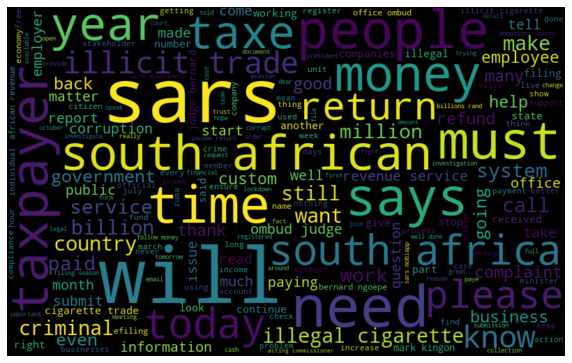
\includegraphics[width=0.5\linewidth]{Wordcloud for frequency of words.png}
    \caption{Enter Caption}
    \label{fig:enter-label}
\end{figure}

\subsubsection{Conclusion}

In conclusion, this chapter on research methodology has focused on the application of machine learning techniques for predicting and recommending hashtags for Twitter social media use of government tax department. Throughout the chapter, we have explored various process leading up to the research methodology, including data preparation, preprocessing, and text mining analysis.  The experiment set up is employing both supervised and unsupervised algorithms machine learning techniques in predicting and recommending hashtags.  For supervised techniques, algorithms such as Support Vector Machines, Random Forest classifiers were trained on the collected data and have been able to make accurate predictions regarding the most relevant hashtags for a given social media post.  The significance of evaluating the performance of supervised models was measured by the accuracy score metrics to compare their performance in comparison.  The evaluation process in training the modes allowed us to fine-tune the final models and enhance their effectiveness in generating accurate hashtag recommendations.

Hashtag recommendation results at a user tweet level summarised below:

The hashtag recommendation system can automatically suggest hashtags to a user while writing a tweet as shown below for the method topic model based.    \textbf{User tweet is: filing season period for filing returns deadline
Recommended tags are: revolt seize filing tomorrow}

All the models are doing better than the dummy classifier to recommend the hashtag for the single tweet (Jaccard score on test set: 44.38 )

"SVM confusion matrix is larger than that of other classifiers,
indicating that the prediction is more accurate and the effect
is better. Finally, the f1-Score obtained by different classifiers
of each label was compared."

The Jaccard score of LDA model on test set is 0.00
The Jaccard score of RFC model on test set is 56.33.
The Accuracy score of RFC model on test set is 0.045.
The Jaccard score of SVM model on test set is 54.20.
The Accuracy score of SVM model on test set is 0.04.
The RFC model is performing better than the SVM model, despite the narrow margins when looking at the Jaccard score, whereas the accuracy score for both is the same.  Due to limitations of adequate metrics to evaluate hashtag recommendation both the accuracy and jaccard scores have not been able to provide a quantifiable measure for the LDA method.  Even with this limitation, the hashtag recommendation system can automatically suggest hashtags to a user while writing a tweet using the LDA topic model based method. 

\subsubsection{Limitations}

Classification-based hashtag recommendation requires less task-specific assumption and engineering in comparison with topic-based hashtag recommendation [80].    \textbf{[80] Weston, J.; Chopra, S.; Adams, K. #TagSpace: Semantic Embeddings from Hashtags; EMNLP; Moschitti, A., Pang, B., Daelemans, W.,Eds.; ACL: Stroudsburg, PA, USA, 2014; pp. 1822–1827.}
Therefore, this study has not identified the superiority of methods between supervised and unsupervised prediction techniques as the classical evaluation metrics may not be useful, however, the study has achieved the  content based hashtag recommendation that has led to possibility of up to 5 hashtags for possible discovery.

